%NOTE: COMPILE IN TERMINAL USING LUALATEX
\documentclass[a4paper,11pt]{standalone}

\usepackage{tikz-feynman}
%\usetikzlibrary{external}             %% Load the `external` library
%\tikzexternalize
%\immediate\write18{mkdir -p pgf-img}
%\tikzexternalize[                     %% Activate externalization
%  system call={                       %% Use lualatex in system call
%    lualatex \tikzexternalcheckshellescape -halt-on-error -interaction=batchmode -jobname="\image" "\texsource" || rm "\image.pdf"
%  },
%]

\begin{document}

%\feynmandiagram [horizontal=b to c]{
%    a -- [fermion,edge label=$b$] b -- [boson,edge label'=$W$] c -- [fermion,edge label=$s$] d,
%    b -- [half left,fermion] c,
%};

%\begin{tikzpicture}
%    \begin{feynman}
%        \vertex (a1);
%        \vertex[right=1.5cm of a1] (a2);
%        \vertex[right=1.5cm of a2] (a3);
%        \vertex[above=1cm of a3] (a4);
%        \vertex[below=1cm of a3] (a5);
%
%        \diagram* {
%            (a1) -- [fermion,edge label=$b$] (a2) -- [boson,edge label'=$W^\pm$] (a5),
%            (a2) -- [fermion,edge label=$c$] (a4),
%        };
%    \end{feynman}
%\end{tikzpicture}
%\quad 
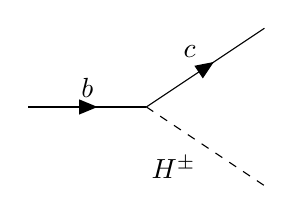
\begin{tikzpicture}
    \begin{feynman}
        \vertex (a1);
        \vertex[right=1.5cm of a1] (a2);
        \vertex[right=1.5cm of a2] (a3);
        \vertex[above=1cm of a3] (a4);
        \vertex[below=1cm of a3] (a5);

        \diagram* {
            (a1) -- [fermion,edge label=$b$] (a2) -- [scalar,edge label'=$H^\pm$] (a5),
            (a2) -- [fermion,edge label=$c$] (a4),
        };
    \end{feynman}
\end{tikzpicture}



\end{document}
